\documentclass[letterpaper,12pt]{article}
\usepackage{tabularx} % extra features for tabular environment
\usepackage{amsmath}  % improve math presentation
\usepackage{graphicx} % takes care of graphic including machinery
\graphicspath{ {images/} }
\usepackage{float}
\usepackage[margin=1in,letterpaper]{geometry} % decreases margins
% \usepackage{cite} % takes care of citations
\usepackage[final]{hyperref} % adds hyper links inside the generated pdf file
\hypersetup{
	colorlinks=true,       % false: boxed links; true: colored links
	linkcolor=blue,        % color of internal links
	citecolor=blue,        % color of links to bibliography
	filecolor=magenta,     % color of file links
	urlcolor=blue         
}

\usepackage{ar}
\usepackage{siunitx}
\usepackage{longtable}
\setlength\LTleft{0pt} 

\begin{document}
\newcommand{\cldat}{\boldsymbol{{c_l}^{2D}}}
\newcommand{\CDp}{C_{D_p}}
\newcommand{\CDi}{C_{D_i}}
\newcommand{\cl}[1]{{c_l}_{\bf #1}}
\newcommand{\cdp}[1]{{c_{d_p}}_{\bf #1}}
\newcommand{\cb}[1]{\left(
	\frac c b 
\right)_{#1}
}
\newcommand{\An}[1]{\bar{A_{#1}}}
\newcommand{\cddat}{\boldsymbol{{c_{d_p}}^{2D}}}
% \newcommand{\CDi}{C_{D_i}}


\title{Glider Optimization with Lifting Line Theory and Airfoil Wind Tunnel Data}
\author{Jean de Becdelievre}
\date{\today}
\maketitle

\section{Nomenclature}

{\renewcommand\arraystretch{1.0}
\noindent\begin{longtable}{@{}l @{\quad : \quad} l@{}}
$W, C_W$  & glider weight, weight coefficient \\
$L, C_L$ & lift, lift coefficient \\
$D,Di,D_p, C_D,C_{Di},C_{D_p}$& drag, induced drag, parasite drag, and respective coefficients \\
$b$ & wing span \\
$S$ & wing area \\
$\AR$ & wing aspect ratio \\
$y$ & span-wise coordinate, ranging from $-b/2$ to $b/2$ \\
$\theta$ & remapped span-wise coordinate ranging from $0$ to $\pi$ \\
$N_{y}$ & Number of span-wise sections \\
$\Gamma(y) \text{ or } \Gamma(\theta)$ & span-wise strength of vortex sheet\\
$A_n$ & nth coefficient of the Fourier expansion of $\Gamma$ \\
$\An{n}$ &  $A_n / A_1$\\
$N_{A}$ & Number of Fourier coefficients considered for $\Gamma$ \\
$c(y) \text{ or } c(\theta)$ & span-wise chord distribution\\
$\cb{k} $ &  chord size of section k along the span, divided by the span $b$\\
$c_l(y) \text{ or } \cl{k}$ & span-wise lift coefficient distribution, lift coefficient at section k\\
$V$ & airspeed \\
$\cddat $ & fit of 2D airfoil data \\
${Re}_{\bf lb}, {Re}_{\bf ub}, {cl}_{\bf lb}, {cl}_{\bf ub}$ & lower and upper bounds on $Re$ and $c_l$, region of validity of  $\cddat$ \\
$Re(y) \text{ or } Re{k}$ & Reynolds number distribution, Reynolds number at spanwise station k \\
$w_{1:Ny}$ & positive quadrature weights allowing to write integrals as discrete sums 
\end{longtable}}


\section{Introduction}

This code aims at optimizing the wing planform and airspeed of a glider of a given weight W and fixed airfoil section for maximum $L/D$.
2D wind tunnel data of the airfoil is available, {\it i.e.} the function
% $\cldat(\alpha, Re)$ and 
$\cddat(c_l, Re)$ are provided for  $c_l \in [\cl{lb}, \cl{ub}]$   and $Re \in [{Re}_{\bf lb}, {Re}_{\bf ub}]$.

Schematically, the optimization problem reads:
\begin{align*}
	& \underset{V, b, c(y), c_l(y)}{\text{minimize}} &  C_D &/ C_L  & \\
	& \text{subject to} 
	&  {C_L}^2 + {C_D}^2 &= {C_W}^2 \quad \text{-} \quad \text{\it gliding flight constraint} \\
	& & \cl{lb} \leq &\cl{k} \leq \cl{ub} \quad \forall k \in [1, N_y] \quad \text{-} \quad \text{\it domain constraint for } \cddat  \\
	& & {Re}_{\bf lb} \leq &{Re_k} \leq {Re}_{\bf ub} \quad \forall k \in [1, N_y] \quad \text{-} \quad \text{\it domain constraint for } \cddat
\end{align*}

First, the optimization problem is described in more details. 
Second, some insights are obtained from considering simple functions for $\cddat$.
Finally, using a neural network fit of 2d airfoil data, the complete problem is solved and results are analyzed.

\section{Fitting Airfoil Data}

The model used here for $\cddat$ comes from a neural network fit of airfoil data from the UIUC database. It is valid for $Re \in [60\,000, 200\,000]$ and $c_l \in [-0.4, 1.25]$. Figure \ref{fig:airfoil_data} shows a plot of the data, as well as contour lines of the neural network fit.

\begin{figure}[H]
	\centering
	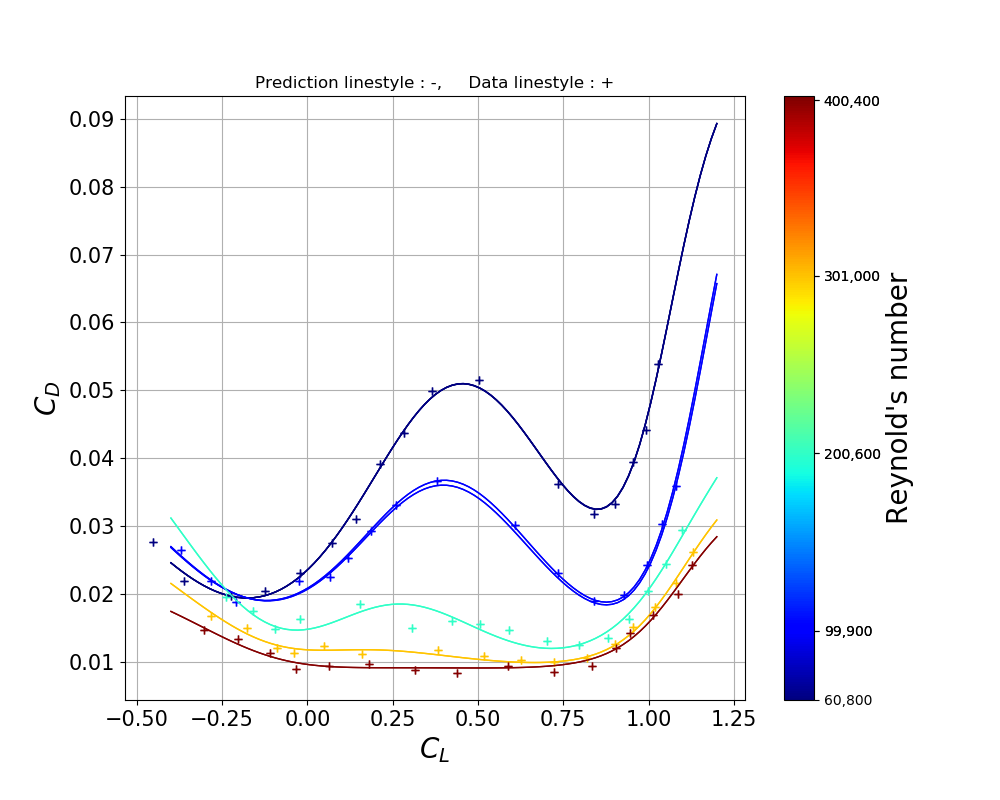
\includegraphics[width=0.8\linewidth]{nn_e231}
	\caption{Neural Network Model of the Airfoil Data}
	\label{fig:airfoil_data}
\end{figure}

\section{Optimization Problem}

\paragraph{Loss Function:}Using the gliding flight constraint, we have:
$$ \frac{{C_L}^2}{{C_D}^2} = \frac{{C_W}^2 - {C_D}^2}{{C_D}^2} = \frac{{C_W}^2}{{C_D}^2} - 1$$
Therefore, minimizing $C_{D} / C_W$  is equivalent to minimizing $C_{D} / C_L$.
Moreover, $C_D$ can be decomposed into lift-induced drag and parasite drag:
$$C_D = \CDp + \CDi$$

\paragraph{Parasite Drag :}Since we can compute the 2D parasite drag using $\cddat$, the total $\CDp$ is obtained with integration.
\begin{align*}
	\CDp &= \frac 1 S \int_{-b/2}^{b/2} c(y) \cddat(c_l(y), Re(y)) dy = \AR \sum_{k=0}^{N_y} w_k \cb{k} \cddat(\cl{k}, Re_k)
\end{align*}
where:
\begin{itemize}
	\item $N_y$ is the number of spanwise panels
	\item $w_{1,\dots, N_y}$ a set of quadrature weights that depend on the spacing and location of the panels, but not on their size or on the total span
	\item $\cb{k} = c_k / b$ is the chord of the kth spanwise panel,  non-dimensionalized by the total span ratio $b$.
\end{itemize} 

\paragraph{Induced Drag:}We use a far field estimate of the induced drag. 
Assuming a planar wake, we use a sine basis expansion of the vortex sheet strength:
$$\Gamma(\theta) = 2bV \sum_{n=1}^{N_a} A_n sin(n \theta)$$
$N_a$ is the order of this expansion.
Using lifting line theory, this give us:
$$\CDi = \frac{C_L^2}{\pi } \left(1+\sum_{n=2}^{N_a} n \An{n}^2\right) $$
where we defined $\An{n} = A_n/A_1$.

\paragraph{Approximate Handling of the Equality Constraint:} We simplify the problem by assuming that the glide angle $\gamma$ is small.
In such case,
\begin{align}
	C_W = \frac{C_L}{\cos \gamma} \approx C_L
	\label{eq:A1}
\end{align}
The validity of the small angle assumption is discussed in appendix \ref{apx:smallangle}.
Instead of solving the original nonlinear constrained problem, we insert the value of $A_1$
 into the objective function. $\pi \AR A_1^2$ appears in the expression of $\CDi$, so we get: 
 \begin{align*}
	\CDi &= \frac{C_W^2}{\pi \AR} \left(1+\sum_{n=2}^{N_a} n \An{n}^2\right)
 \end{align*}

 \paragraph{Objective Function:}Putting together all of the above, we obtain the following objective function:
$$\frac{C_D}{C_W} = \frac{C_W}{\pi \AR} \left(1+\sum_{n=2}^{N_a} n \An{n}^2\right) +
\frac {\AR} {C_W} \sum_{k=0}^{N_y} w_k \cb{k} \cddat(\cl{k}, Re_k) $$
Replacing $C_W$ by its value, we actually optimize:
$$\frac{4W}{\pi \rho^2 (Vb)^2} \left(1+\sum_{n=2}^{N_a} n \An{n}^2\right) +
(Vb)^2 \sum_{k=0}^{N_y} w_k \cb{k} \cddat(\cl{k}, Re_k) $$


\paragraph{Reynolds and Lift Coefficient Bounds:} We can write the Reynolds number $Re_{k}$ and the lift coefficient $\cl{k}$ at the local section k as a function of other variables used previously:

$$Re_{k} = \frac{\rho}{\nu}\cb{k}(Vb) $$

$$
	\cl{k} = \frac{8W}{\pi \rho (Vb)^2\cb{k}} \left(\sin(\theta_k) + \sum_{n=2}^{N_a} \An{n} \sin(n \theta_k)\right)
$$


The collected optimization problem is written and analyzed in the next section.

\section{Optimization Problem Insights and Discussion}

\begin{align*}
	& \underset{Vb, \cb{1:N_y}, \An{2:N_a}}{\text{minimize}}  &
	\frac{4W}{\pi \rho^2 (Vb)^2} \left(1+\sum_{n=2}^{N_a} n \An{n}^2\right) &+
(Vb)^2 \sum_{k=0}^{N_y} w_k \cb{k} \cddat(\cl{k}, Re_k) & \\
	& \text{subject to} & \cl{lb} \leq &\cl{k} \leq \cl{ub} \quad \forall k \in [1, N_y] \\
	& & {Re}_{\bf lb} \leq &{Re_k} \leq {Re}_{\bf ub} \quad \forall k \in [1, N_y] 
\end{align*}

with:
$$Re_{k} = \frac{\rho}{\nu}\cb{k}(Vb) $$

$$
	\cl{k} = \frac{8W}{\pi \rho (Vb)^2\cb{k}} \left(\sin(\theta_k) + \sum_{n=2}^{N_a} \An{n} \sin(n \theta_k)\right)
$$

\paragraph{Design Variables:} The first interesting note is that the optimization of the planform and airspeed only requires:
\begin{itemize}
	\item $(Vb)^2$ which is the only place where the airspeed appears. Note that we could equivalently use $C_W / \AR$, which makes it obvious that this design variable is tightly connected to the nominal $C_L$.
	\item $\cb{1:N_y}$ is simply related to the planform shape
	\item $\An{2:N_a}$ describes the lift distribution. Note that $A_1$ is not a design variable, it is directly set by the value of $C_W / (\pi \AR)$.
\end{itemize}
 This set of variables is not sufficient to recover the wing dimensions, or even the airspeed. Once the optimization has converged, choosing either a span value $b$, an airspeed $V$, or the chord $c_k$ of any of the chord sections allows to recover the full dimensional planform shape.

\paragraph{Feasibility Range:} This problem is feasible for any weight $W$, air density $\rho$ or viscosity $\nu$. As $W$ varies, it becomes more complicated to make the $c_l$ bound. But, even though there is a bound on $\cb{k}(Vb)$ (from the bound on Re), there is no bound on $\cb{k}(Vb)^2$ in the current format. Therefore we can always find a set of $\cb{k}(Vb)^2$ such that the $c_l$ bound is respected.

\section{Insights from Simplified 2D Section Models}
\subsection{Constant $\cddat$}

Let us assume:
$$\cddat(\cl, Re) = \cdp{} \text{\it (constant)}$$
Then the optimization problem becomes:

\begin{align*}
	& \underset{Vb, \cb{1:N_y}, \An{2:N_a}}{\text{minimize}}  &
	\frac{4W}{\pi \rho^2 (Vb)^2} \left(1+\sum_{n=2}^{N_a} n \An{n}^2\right) &+
(Vb)^2 \sum_{k=0}^{N_y} w_k \cb{k} \cdp{}  & \\
	& \text{subject to} & \cl{lb} \leq &\cl{k} \leq \cl{ub} \quad \forall k \in [1, N_y] \\
	& & {Re}_{\bf lb} \leq &{Re_k} \leq {Re}_{\bf ub} \quad \forall k \in [1, N_y] 
\end{align*}

We can see that:
\begin{itemize}
	\item $\An{2:N_a} \rightarrow 0 $ to minimize induced drag
	\item The chord elements $\cb{1:N_y}$ will all tend to 0, or to their minimal value allowed by the Re bound.
	\item $Vb$ will reach a finite, non-zero optimal value (to the extent that this makes sense if $\cb{1:N_y} = 0$)
\end{itemize}
Without a proper 2D section model, this problem has limited interest: the optimal $L/D$ is always obtained at the minimal allowed chord.

\subsection{Flat Plate Model}

We now assume:
$$\cddat(\cl, Re) = \cdp{} Re^{-\eta} = \cdp{}
\left(\frac{\rho}{\nu}\cb{k}(Vb)\right)^{-\eta}$$
Typically, for a turbulent flat plate, we would have $\eta=0.2$.
Then we obtain:
\begin{align*}
	& \underset{Vb, \cb{1:N_y}, \An{2:N_a}}{\text{minimize}}  &
	\frac{4W}{\pi \rho^2 (Vb)^2} \left(1+\sum_{n=2}^{N_a} n \An{n}^2\right) &+
	(Vb)^{2-\eta} \sum_{k=0}^{N_y} w_k \cb{k}^{1-\eta} \left(\frac{\rho}{\nu}\right)^{-\eta}\cdp{}  & \\
	& \text{subject to} & \cl{lb} \leq &\cl{k} \leq \cl{ub} \quad \forall k \in [1, N_y] \\
	& & {Re}_{\bf lb} \leq &{Re_k} \leq {Re}_{\bf ub} \quad \forall k \in [1, N_y] 
\end{align*}
%
In such case:
\begin{itemize}
	\item There still is no incentive to do anything else than an elliptic lift distribution: $\An{2:N_a} \rightarrow 0 $ to minimize induced drag.
	\item  The chord elements $\cb{1:N_y}$ will all tend to 0 for any value of $\eta$ smaller than 1.
	\item Again, $Vb$ will reach a finite, non-zero optimal value unless $\eta$ becomes bigger than 2.
\end{itemize}
%
Here we can see that this problem starts to make sense if the $\CDp$ penalty for decreasing the chord is more than linear in $1/\cb{k}$, i.e. $\eta \geq 1$. This is not likely to come from a variation of $\CDp$ with the Reynolds number, but could come from a variation with $c_l$.

\subsection{Flat Plate with Quadratic $C_L$ Dependency}

We now assume:
\begin{align}
	\label{eq:simple_model}
	\cddat(\cl, Re) &= \cdp{0} Re^{-\eta} + \cdp{1} \cl{}^2  \\
	% &= \cdp{0}\left(\frac{\rho}{\nu}\cb{k}(Vb)\right)^{-\eta} + 
	% \cdp{1}\left(\frac{8W}{\pi \rho (Vb)^2\cb{k}} \left(\sin(\theta_k) + \sum_{n=2}^{N_a} \An{n} \sin(n \theta_k)\right)\right)^2 ) \\
	&= \cdp{0}'\cb{k}^{-\eta}(Vb)^{-\eta}+ 
	\cdp{1}'\frac{W^2}{(Vb)^4\cb{k}^2} \left(\sin(\theta_k) + \sum_{n=2}^{N_a} \An{n} \sin(n \theta_k)\right)^2 
	\nonumber
\end{align}
where several constant terms are regrouped under $\cdp{0}'$ and $\cdp{1}'$.
The terms of the objective function can be split in the following way:
\begin{subequations}
	\begin{align}
		& \frac{4W}{\pi \rho^2 (Vb)^2} \left(1+\sum_{n=2}^{N_a} n \An{n}^2\right) & {
			\text{span-dependent induced drag} 
		} \label{eq:fpq_di}&\\ 
		& + {\cdp{0}'(Vb)^{2-\eta} \sum_{k=0}^{N_y} w_k \cb{k}^{1-\eta}} & {
			Re\text{-dependent parasite drag}
		} & \label{eq:fpq_re}\\
		& + W^2{\cdp{1}'\sum_{k=0}^{N_y} w_k \cb{k}^{-1}(Vb)^{-2}
		\left(\sin(\theta_k) + \sum_{n=2}^{N_a} \An{n} \sin(n \theta_k)\right)^2 } & {
			c_l\text{-dependent parasite drag}
		}& \label{eq:fpq_cl}
		\end{align}	
\end{subequations}
%
The following behavior is observed:
\begin{itemize}
	\item  The chord elements $\cb{1:N_y}$ do not tend to 0 anymore. The penalty for increasing $c_l$ \ref{eq:fpq_cl} and reducing Re \ref{eq:fpq_re} act together to prevent it. We note that the $c_l$ penalty is is far stronger.
	\item Again, $Vb$ will reach a finite, non-zero optimal value unless $\eta$ becomes bigger than 2. The optimal of $Vb$ is much higher what is estimated in the previous case because of the incentive from \ref{eq:fpq_cl} to reduce $c_l$.
	\item The effect of $\An{2:N_a}$ from \ref{eq:fpq_cl} dominates the induced drag penalty  \ref{eq:fpq_di} for a non-elliptical wing distribution.  $\An{2:N_a}$ is mostly chosen in order to minimize the average $c_l^2$.
\end{itemize}
%
As the airplane weight varies, we observe:
\begin{itemize}
	\item For small W, \ref{eq:fpq_re} has main biggest role, which will push for shorter chord, and higher $Vb$
	\item For slightly higher W, the penalty on lift per unit span \ref{eq:fpq_di} kicks in, and higher spans are encouraged. 
	\item At high W, the dominant term is \ref{eq:fpq_cl}. Bigger chords, lower $Vb$ and non-elliptic lift distribution are promoted.
\end{itemize}

\subsection{Results With Polynomial Fit}

A fit of the form show in equation \ref{eq:simple_model} of the 2D data shown on Figure \ref{fig:airfoil_data} is realized. 

The fit captures both essential facts that $\cdp{}$ decreases with $Re$, and that there is a sharp increase in $c_l$ after approximately $c_l = 0.8$.




\subsection{Gathered insights}

This section illustrates the dramatic changes in the optimal solution that can occur when changing the 2D section parasite drag model.
Especially, not taking into account $c_l$ dependance leads to unrealistic solutions, where the optimal $L/D$ only happens at the minimum chord.

A physical solution only happens when a penalty on 2d section $c_l$ is included, and the $c_l$ dependance has a major impact on the final solution. This motivates the use of an accurate 2d section model.


\appendix

\section{Validity of the small angle assumptions}
\label{apx:smallangle}
TBD

\end{document}


